\documentclass{report}

\usepackage[utf8]{inputenc}  
\usepackage[T1]{fontenc}    
\usepackage{graphicx}
\usepackage{listings}

\lstset{
  language=Caml
}

\title{TER - Rendu 1}
\author{Emile Cadorel, Guillaume Gas, Jimmy Furet, Valentin Bouziat}
\date{11 mars 2016}

\begin{document}
\maketitle

\chapter{Introduction}

\section{La Programmation GPGPU}
La programmation GPGPU\cite{refProgGPGPU} (General Purpose on Graphic Processing Units), est un principe informatique visant à utiliser le processeur graphique comme processeur de calcul générique. L’objectif étant de bénéficier de l’architecture massivement parallèle d’un processeur graphique et ainsi résoudre des problèmes pour lesquels nous avons des algorithmes parallèles efficaces.\newline

En effet le processeur graphique possède une capacité de calcul beaucoup plus grande que celle d’un processeur classique. Pour peu qu’il existe un algorithme parallèle pour un problème donné. La programmation GPGPU n’est applicable qu’avec utilisation des pilotes et des bibliothèques associées. Ces pilotes et bibliothèques généralement proposés par les constructeurs de processeur (ex: Intel, Nvidia, …) permettent la programmation sur la carte graphique pour des informaticiens chevronnés.\newline 

Il existe deux piliers dans la programmation GPGPU, OpenCL : bibliothèques ouvertes par Khronos Group, et Cuda : développée par Nvidia et nécessitant un GPU Nvidia.
Les bibliothèques proposent la création de noyaux  (kernel), fonction exécuté sur le GPU, la gestion de mémoire sur le GPU et le passage de données entre la RAM du GPU et la RAM du CPU.\newline

La programmation GPGPU étant d’assez bas-niveaux, il existe des bibliothèques permettant d’abstraire certains principes, comme la gestion mémoire. 

\section{SPOC}
SPOC\cite{refSpoc}, Stream Processing with OCaml est une bibliothèque qui propose une abstraction pour la programmation GPGPU. Son principal but est de fournir une solution portable, multi-GPGPU, et hétérogène tout en gardant de hautes performances.\newline

Elle permet ainsi l’utilisation des systèmes Cuda/OpenCL avec OCaml, l’unification de ces deux API se faisant via une liaison dynamique, ainsi que d’abstraire également les transferts de données entre le CPU et la carte graphique.\newline

Enfin, elle permet aussi d’utiliser le typage statique afin de vérifier les noyaux de calcul, écrits en Sarek.\newline

Il existe deux solutions afin d’exprimer les noyaux :
\begin{itemize}
  
\item Sarek : un langage proche de OCaml. Sarek est compatible avec les bibliothèques existantes, ses performances sont facilement prévisibles et optimisables.
  
\item L’interopérabilité avec les noyaux Cuda/OpenCL : permet de réaliser des optimisations supplémentaires, compatible avec les bibliothèques actuelles, mais moins robuste que Sarek.


\end{itemize}


\section{Les Squelettes de programmation}
Les squelettes de programmation\cite{refSkeleton} sont une forme de programmation, ou il existe des éléments générique pré-définis - tel que map, reduce, farm, pipe etc... Ces squelettes peuvent être personnalisé grâce à du code utilisateur.\newline

Les squelettes permettent une abstraction de haut niveau et aident les utilisateurs à implémenter des algorithmes complexe comme les algorithmes parallèles. Les algorithmes suivant sont généralement implémenté en tant que squelette dans les bibliothèque de programmation GPGPU.\newline

Afin de mieux comprendre le but de notre travail, nous avons fait des recherches sur la programmation de tels squelettes sur internet. Nous avons ainsi pris exemple sur deux bibliothèques qui semblent reprendre les concepts nous intéressent : Thrust, développée par Nvidia, et SkePU.\newline

\subsection{Thrust}
Cette bibliothèque de templates C++ pour Cuda est basée sur la STL (Standard Template Library). Elle permet l’utilisation d’algorithmes parallèles avec un minimum de code. Ainsi, on retrouve les algorithmes suivant :

\begin{itemize}
\item Transformations : applique une opération d’un “set” de données et met le résultat dans un “set” de destination. 
\item Réductions : utilise une opération binaire pour réduire une entrée en une unique valeur. 
\item Prefix-Sums : ou opération “scan” permet par exemple, sur un tableau en entrée, d’obtenir en sortie un tableau avec les sommes cumulées.
\item Reordering : permet d’arranger ou partitionner des données selon des prédicats de test.
\item Sort : tri un ensemble d’élément à l’aide d’une relation d’ordre donné.
\end{itemize}

\subsection{SkePU}
Librairie de templates C++ mettant à disposition un ensemble de squelettes génériques.

\begin{itemize}
\item Map\cite{refMap} - applique une fonction donnée à toutes les entrées d’un tableau.
\item MapReduce - réduction d’un tableau dans une variable, en fonction d’un operateur donné.
\item MapOverlap
\item MapArray
\item Generate
\item Scan
\item ...
\end{itemize}

\chapter{Présentation du sujet}

\section{Introduction au domaine}
La programmation GPGPU permet de profiter de l’architecture massivement parallèle du GPU. Le GPU possède une architecture SIMD (Single Instruction Multiple Data), proposant de nombreuse unités de calcul.\newline

Le GPU est decoupée en plusieurs TCP (Texture Processing Cluster), eux-même découpés en plusieurs SM. Les SM (Streaming Multi-processor) possèdent une mémoire locale, ils possèdent plusieurs SP (Streaming Processor) permettant des calculs sur nombres flottants, ainsi que des unités SFU (Special Function) permettant le calcul de fonctions spécifiques - cos, sin… . Une mémoire globale est la disposition de chacun des clusters mais est beaucoup plus lente que leur mémoire locale.

\begin{figure}[!h]
\begin{center}
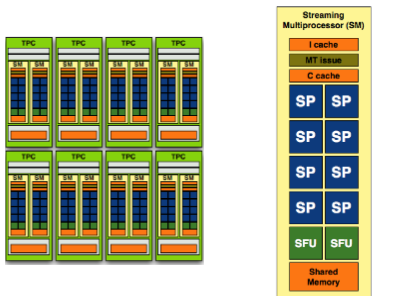
\includegraphics[height=150]{image2.png}
\end{center}
\caption{Représentation d’une architecture GPU - ref : Introduction à la programmation GPGPU avec Cuda, Mathias Bourgoin & Sylvain Jubertie.}
\label{test}
\end{figure} \newline

L’architecture d’un GPU étant SIMD (Single Intruction Multiple Data), il n’est pas conseillé de créer des programmes complexes proposant beaucoup de conditions, ce qui ferait perdre l'intérêt parallèle de la carte, en effet certains coeurs seraient en attente la plupart du temps. 

\section{Analyse de l'existant}
Actuellement, la version de SPOC disponible permet déjà d’effectuer des calculs sur la carte graphique, que ce soit en utilisant Cuda ou OpenCL. Elle nous donne également le choix entre l’utilisation de noyaux Sarek ou bien en Cuda/OpenCL. De plus, SPOC met à notre disposition trois bibliothèques, Sarek en faisant partie, les autres permettant d’utiliser des kernels ecrits en cuda, ou opencl.\newline

Sarek est un langage interne à Spoc permettant de définir des kernel dans un langage proche de ocaml. Ce langage est compilé par Kirc, qui en génère un code exécutable soit par cuda, soit par opencl en fonction de l’architecture de l’ordinateur hôte préalablement detectée.

Spoc propose aussi une bibliothèque Compose, celle-ci permet déjà d’utiliser 3 squelette - Map, Reduce et Pipe. Ces squelettes prennent en paramètre une fonction kernel codé en Cuda ou en Opencl. Le nombres de thread et de block de calcul à créer sur le GPU sont définis de matière automatique. 
  
\chapter{Objectifs et organisation}

Notre travail tout au long du projet consistera en :
\begin{itemize}
\item Modifier le langage Sarek.
\end{itemize}

Pour créer des squelettes pour Spoc, il faudra modifier le compilateur de Sarek, Kirc. Ajouter un élément de syntaxe au langage Sarek, cet élément sera ensuite remplacé par les fonctions créées par les utilisateurs de Spoc. 

\begin{lstlisting}
let foo = fun a -> a + 1;

let map = kern a b n ->
  let open Std in
  let open Skel in
  let idx = global_thread_in in
  if idx < n then
    b.[<idx>] <- { a.[<idx>] }
;;

Kirc.gen map foo;; 
\end{lstlisting}

Le code ci dessus sera alors transformé de la sorte :

\begin{lstlisting}
let map = kern a b n ->
  let open Std in
  let idx = global_thread_in in
  if idx < n then
    b.[<idx>] <- a.[<idx>] + 1;;
\end{lstlisting}

Nous pourrons aussi, définir de nouveaux squelettes pour la bibliothèque d’extension Compose, mais l’utilisateur devra alors connaître les kernels Cuda ou OpenCL pour les utiliser. 

\begin{itemize}
\item Créer des squelettes, pour Sarek.
\item Effectuer des test de performances sur des calculs parallèlisés en les comparant à une exécution séquentielle, mais aussi comparer nos squelettes à d’autres squelettes présent dans d’autres bibliothèques GPGPU.
\item Réaliser une documentation.
\end{itemize}

\bibliographystyle{unsrt}
\bibliography{biblio}

\end{document}
